\documentclass[12pt]{article}

\usepackage[utf8]{inputenc}
\usepackage{geometry}
\geometry{a4paper, margin=1in}
\usepackage{graphicx}
\usepackage{hyperref}
\usepackage{fancyhdr}
\usepackage{listings} 
\usepackage{float}
\usepackage{xcolor}

\lstdefinelanguage{yaml}{
    keywords={true, false, null, yes, no},
    comment=[l]{\#},
    morestring=[b]',
    morestring=[b]",
    stringstyle=\color{red},
    keywordstyle=\color{blue}\bfseries,
    identifierstyle=\color{black},
    commentstyle=\color{green}\itshape,
    sensitive=false
}

\lstdefinelanguage{vim}{
    keywords={function, endfunction, if, endif, let, set, call, return, elseif},
    keywordstyle=\color{blue}\bfseries,
    sensitive=true,
    morecomment=[l]{\"},   
    morestring=[b]',       
    morestring=[b]"        
}

\lstdefinelanguage{C}{
    keywords={int, float, if, else, while, for, return, void, char, malloc, free, sizeof, struct, NULL},
    keywordstyle=\color{blue}\bfseries,
    sensitive=true,
    morecomment=[l]{//},   
    morecomment=[s]{/*}{*/}, 
    commentstyle=\color{green}\itshape,
    morestring=[b]",       
    morestring=[b]'        
}

\lstdefinelanguage{bash}{
    keywords={if, then, else, elif, fi, for, while, do, done, case, esac, function},
    keywordstyle=\color{blue}\bfseries,
    ndkeywords={echo, exit, read, printf, cd, pwd, mkdir, rm, touch, cp, mv},
    ndkeywordstyle=\color{teal}\bfseries,
    sensitive=true,
    morecomment=[l]{\#},   
    commentstyle=\color{green}\itshape,
    morestring=[b]",       
    morestring=[b]'
}


\lstset{
    basicstyle=\ttfamily\footnotesize, 
    frame=lines, 
    backgroundcolor=\color{white}, 
    rulecolor=\color{black}, 
    tabsize=2, 
    showspaces=false, 
    showstringspaces=false, 
    showtabs=false, 
    breaklines=true, 
    breakatwhitespace=true 
}


\setlength{\headheight}{15pt}
\pagestyle{fancy}
\fancyhf{}
\rhead{Computer Workshop Course}
\lhead{Final Assignment}
\rfoot{Page \thepage}

\title{
    \vspace{2in}
    \textbf{Final Assignment :}\\
    \textbf{Integration of Tools and Practices}\\
    \large Iran University of Science and Technology\\
    \large Department of Computer Engineering\\
    \vspace{2in}
}

\author{
    \vspace{0.5in}
    Qazal Arabali\\
    Computer Workshop\\
    \vspace{0.5in}
}

\date{January 25, 2025}
\begin{document}

\begin{titlepage}
    \maketitle
    \thispagestyle{empty}
\end{titlepage}

\newpage

\tableofcontents
\newpage

\section{Git and GitHub}
    \subsection{Repository Initialization and Commits}
    
To initialize the repository and make the first commits, the following steps were taken :

\begin{enumerate}
    \item Logged into \textbf{GitHub} and created a new repository named :
    \texttt{CW\_Final\_Assignment}
    
    \item Configured the repository settings :
    \begin{itemize}
        \item Set the repository visibility to \textbf{Public}.
        \item Checked the box: \texttt{Initialize this repository with a README}.
    \end{itemize}

    \item Cloned the repository to the local system using the command :
    \begin{lstlisting}
    git clone https://github.com/username/CW_Final_Assignment
    \end{lstlisting}

    \item Navigated to the cloned repository directory :
    \begin{lstlisting}
    cd CW_Final_Assignment
    \end{lstlisting}

    \item Created a new LaTeX file named \texttt{CW\_Final\_Assignment.tex} with the initial structure.

    \item Staged and committed the new file:
    \begin{lstlisting}
    git add CW_Final_Assignment.tex
    git commit -m "Added initial LaTeX file"
    \end{lstlisting}

    \item Pushed the changes to the GitHub repository :
    \begin{lstlisting}
    git push
    \end{lstlisting}
\end{enumerate}

\subsection{GitHub Actions for LaTeX Compilation}

To streamline the process of compiling the LaTeX document and managing different stages of updates, two distinct GitHub Actions workflows were created :

\begin{itemize}
    \item \textbf{Workflow for Intermediate Versions :}
    This workflow compiles the LaTeX document and uploads the resulting PDF as an \textbf{Artifact}. It is used for minor updates or ongoing progress, ensuring the document is accessible for review without cluttering the Releases section.
    
    \item \textbf{Workflow for Major Releases :}
    This workflow compiles the LaTeX document and publishes the resulting PDF as part of a \textbf{GitHub Release}. It is triggered only for significant updates or finalized versions to provide stable releases for public access.
\end{itemize}

\subsubsection*{Workflow for Intermediate Versions (Artifact Only)}

For intermediate updates or minor progress, the LaTeX document is compiled and uploaded as an \textbf{Artifact}. This ensures that ongoing work is accessible for review and testing without cluttering the Releases section.

\begin{enumerate}
    \item \textbf{Trigger :} This workflow runs on every \texttt{push} to the \texttt{main} branch.
    \item \textbf{Outcome :} The compiled PDF is stored in the \textbf{Actions > Artifacts} section for download.
    \item \textbf{Workflow Configuration :}
    \begin{lstlisting}[language=yaml]
        name: Compile LaTeX and Upload Artifact
        
        on:
          push:
            branches:
              - main
        
        jobs:
          build_latex:
            runs-on: ubuntu-latest
            steps:
              - name: Checkout Repository
                uses: actions/checkout@v3
        
              - name: Compile LaTeX Document
                uses: xu-cheng/latex-action@v2
                with:
                  root_file: CW_Final_Assignment.tex
        
              - name: Upload Compiled PDF as Artifact
                uses: actions/upload-artifact@v3
                with:
                  name: CW_Final_Assignment
                  path: ./CW_Final_Assignment.pdf
        \end{lstlisting}
        
\end{enumerate}

\subsubsection*{Workflow for Major Releases}

For significant updates or final versions, the LaTeX document is compiled, and the resulting PDF is published as part of a \textbf{GitHub Release}. This approach ensures that only stable and finalized versions are available in the Releases section.

\begin{enumerate}
    \item \textbf{Trigger :} This workflow runs on every \texttt{push} of a Git tag in the format \texttt{x.x.x} (e.g., \texttt{1.0.0}).
    \item \textbf{Outcome :} The compiled PDF is attached to a new Release in the \textbf{Releases} section.
    \item \textbf{Workflow Configuration :}
    \begin{lstlisting}[language=yaml]
        name: Release Compiled PDF
        
        on:
          push:
            tags:
              - '*.*.*'
        
        jobs:
          build_latex:
            permissions: write-all
            runs-on: ubuntu-latest
            steps:
              - name: Checkout Repository
                uses: actions/checkout@v3
        
              - name: Compile LaTeX Document
                uses: xu-cheng/latex-action@v2
                with:
                  root_file: CW_Final_Assignment.tex
        
              - name: Create Release
                id: create_release
                uses: actions/create-release@v1
                env:
                  GITHUB_TOKEN: ${{ secrets.GITHUB_TOKEN }}
                with:
                  tag_name: ${{ github.ref }}
                  release_name: Release ${{ github.ref }}
                  draft: false
                  prerelease: false
        
              - name: Upload Release Asset
                id: upload_release_asset
                uses: actions/upload-release-asset@v1
                env:
                  GITHUB_TOKEN: ${{ secrets.GITHUB_TOKEN }}
                with:
                  upload_url: ${{ steps.create_release.outputs.upload_url }}
                  asset_path: ./CW_Final_Assignment.pdf
                  asset_name: CW_Final_Assignment.pdf
                  asset_content_type: application/pdf
    \end{lstlisting}
        
\end{enumerate}

\section{Exploration Tasks}
    \subsection{Vim Advanced Features}
    Here are three advanced features of Vim that go beyond the topics covered in class :

    \subsubsection*{Registers}

    Registers in Vim allow you to store multiple pieces of text in separate "clipboard" areas and retrieve them as needed. This can enhance productivity when working with multiple text snippets.

    \begin{itemize}
        \item To copy text to a specific register, use :
        \begin{lstlisting}
        "aY  # Copy text to register 'a'.
        \end{lstlisting}
        \item To paste text from a specific register, use :
        \begin{lstlisting}
        "ap  # Paste text from register 'a'.
        \end{lstlisting}
    \end{itemize}

    \subsubsection*{Macros}

    Macros enable you to record and replay a series of commands, making repetitive tasks easier.

    \begin{itemize}
        \item To start recording a macro :
        \begin{lstlisting}
        q{register}  # Start recording to a register (e.g., 'a').
        \end{lstlisting}
        \item To stop recording :
        \begin{lstlisting}
        q
        \end{lstlisting}
        \item To play back the macro :
        \begin{lstlisting}
        @{register}  # Play the macro stored in the register.
        \end{lstlisting}
    \end{itemize}

    \subsubsection*{Persistent Undo}

    Persistent Undo allows you to keep the undo history of a file even after closing and reopening Vim.

    \begin{itemize}
        \item To enable persistent undo, add the following to your `.vimrc` :
        \begin{lstlisting}[language=vim]
        set undofile
        set undodir=~/.vim/undodir
        \end{lstlisting}
        \item Once enabled, you can navigate the undo history using :
        \begin{lstlisting}
        u       # Undo the last change.
        Ctrl-r  # Redo the last undone change.
        \end{lstlisting}
    \end{itemize}



    \subsection{Memory profiling}
        \subsubsection{Memory Leak}

            A \textbf{memory leak} occurs when a program allocates memory during its execution but fails to release it after it is no longer needed. Over time, this can lead to increased memory usage and potentially cause the program or the system to run out of memory. Memory leaks typically happen due to :

            \begin{itemize}
                \item Forgetting to free dynamically allocated memory.
                \item Retaining references to objects that are no longer needed, preventing their deallocation.
                \item Errors in pointer management, such as overwriting pointers without freeing the associated memory.
            \end{itemize}
            
            For example, in C programming, a memory leak might look like this :
            \begin{lstlisting}[language=c]
            #include <stdlib.h>
            
            int main() {
                int *ptr = (int *)malloc(sizeof(int) * 10); // Memory allocated
                // Forgot to free the allocated memory
                return 0; // Memory is leaked here
            }
            \end{lstlisting}
            
            To prevent memory leaks :
            \begin{itemize}
                \item Always release memory using \texttt{free()} in C or \texttt{delete} in C++.
                \item Use memory profiling tools, such as \textbf{Valgrind}, to identify and fix leaks.
                \item Adopt good coding practices, such as using smart pointers in modern C++.
            \end{itemize}




        \subsubsection{Memory profilers}

            \textbf{Valgrind : Purpose and How It Helps with Memory Leaks}
            
            Valgrind is a powerful instrumentation framework for building dynamic analysis tools. The most commonly used tool within the Valgrind suite is \textbf{Memcheck}, which helps detect memory-related issues in programs, such as memory leaks, use of uninitialized memory, and accessing invalid memory locations.
            
            \paragraph{Purpose of Valgrind}
            The primary purpose of Valgrind is to ensure memory correctness in programs by :
            \begin{itemize}
                \item Detecting memory leaks that occur when dynamically allocated memory is not properly freed.
                \item Identifying invalid memory accesses, such as reading or writing outside the bounds of an array.
                \item Detecting the use of uninitialized memory, which can lead to unpredictable behavior.
                \item Helping developers understand and debug complex memory issues.
            \end{itemize}
            
            \paragraph{How Valgrind Helps with Memory Leaks}
            Valgrind identifies memory leaks by monitoring all dynamic memory allocations and deallocations. At the end of the program's execution, it reports:
            \begin{itemize}
                \item \textbf{Definite Leaks} : Memory that was allocated but never freed.
                \item \textbf{Indirect Leaks} : Memory that is still reachable through pointers but was not explicitly freed.
                \item \textbf{Suppressed Errors} : Issues that are configured to be ignored.
            \end{itemize}
            
            Using Valgrind, developers can pinpoint the exact location in the code where memory issues occur, making it easier to fix the problem.
            
            \paragraph{Example Usage of Valgrind}
            Below is an example of how to use Valgrind to detect memory leaks in a C program :
            
            \begin{lstlisting}[language=C]
            #include <stdlib.h>
            #include <stdio.h>
            
            int main() {
                int *array = (int *)malloc(10 * sizeof(int)); // Allocate memory
                array[0] = 42; // Use the memory
                // Memory is not freed intentionally
                return 0;
            }
            \end{lstlisting}
            \vspace*{2cm}
            To run the program with Valgrind :
            
            \begin{lstlisting}[language=bash]
            valgrind --leak-check=full --track-origins=yes ./my_program
            \end{lstlisting}
            \vspace*{2cm}
            Example output :
            
            \begin{lstlisting}
                ==12345== Memcheck, a memory error detector
                ==12345== LEAK SUMMARY:
                ==12345==    definitely lost: 40 bytes in 1 blocks
                ==12345==    indirectly lost: 0 bytes in 0 blocks
                ==12345==    possibly lost: 0 bytes in 0 blocks
                ==12345==    still reachable: 0 bytes in 0 blocks
                ==12345==         suppressed: 0 bytes in 0 blocks
            \end{lstlisting}
            
            \paragraph{Benefits of Using Valgrind}
            \begin{itemize}
                \item Simplifies debugging of memory-related issues.
                \item Provides detailed error reports for quicker resolution.
                \item Helps improve the stability and performance of software by ensuring proper memory management.
            \end{itemize}
            
            \paragraph{Best Practices When Using Valgrind}
            \begin{itemize}
                \item Compile programs with debugging symbols (\texttt{-g} flag) for detailed reports.
                \item Regularly run Valgrind during development to catch issues early.
                \item Suppress known or irrelevant errors using suppression files.
            \end{itemize}
            

    \subsection{GNU/Linux Bash Scripting}
        \subsubsection{fzf}
            \textbf{What is fuzzy searching ?}

            Fuzzy searching is a technique used to find approximate matches to a given query string, rather than requiring an exact match. This is particularly useful when the user does not remember the full or exact input, or when there are minor typos. Instead of matching exact characters in the correct sequence, fuzzy searching prioritizes likely matches based on the query and displays them in an interactive interface.
            
            \textbf{fzf} (Fuzzy Finder) is a command-line tool that provides an efficient way to perform fuzzy searching. It is highly customizable, interactive, and lightweight. It can be used to search for files, commands, or any list of items in the terminal.
            
            \paragraph{Example usage :}
            Suppose you want to search for a file in a directory. With \texttt{fzf}, you simply type a part of the file name, and it will display all matches dynamically as you type.
            
            \begin{lstlisting}[language=bash]
            # Search for a file
            fzf
            
            # Example : Combining with find command
            find . -type f | fzf
            \end{lstlisting}
            
            \paragraph{Key Features of fzf :}
            \begin{itemize}
                \item Interactive interface that displays results as you type.
                \item Supports integration with other tools and commands.
                \item Can be used in combination with pipes for filtering outputs.
                \item Lightweight and customizable with various options.
            \end{itemize}


            \textbf{Install fzf and Explanation of \texttt{ls | fzf}}

            To install \texttt{fzf} on the system, the following steps were taken :

            \begin{enumerate}
                \item Updated the package list :
                \begin{lstlisting}[language=bash]
                sudo apt update
                \end{lstlisting}

                \item Installed \texttt{fzf} using the \texttt{apt} package manager :
                \begin{lstlisting}[language=bash]
                sudo apt install fzf
                \end{lstlisting}

                \item Verified the installation by checking the version :
                \begin{lstlisting}[language=bash]
                fzf --version
                \end{lstlisting}
            \end{enumerate}

            \textbf{Result of Installation :}

            \begin{figure}[H]
                \centering
                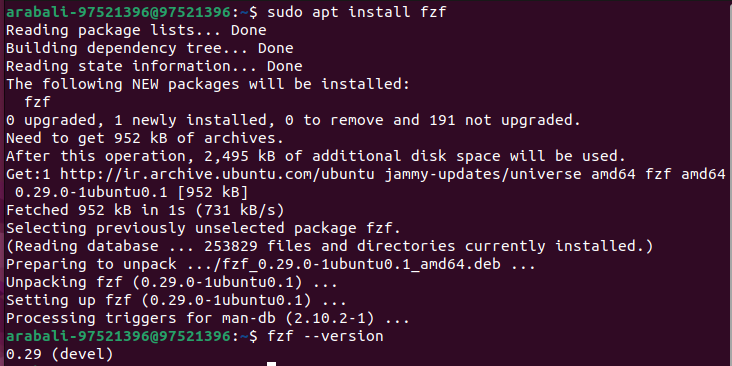
\includegraphics[width=\textwidth]{assets/pictures/installation_of_fzf.png}
                \caption{Successful installation of \texttt{fzf}.}
            \end{figure}
            
            \textbf{Explanation of \texttt{ls | fzf} :}

            This command integrates the output of \texttt{ls} with the fuzzy finder tool, \texttt{fzf}, to dynamically and interactively search for files or directories. Here's how it works:

            \begin{enumerate}
                \item \texttt{ls} lists all files and directories in the current folder.
                \item The output is piped to \texttt{fzf}, which allows the user to type part of a file or directory name.
                \item \texttt{fzf} filters the results interactively and highlights the matching entries.
            \end{enumerate}

            \textbf{Demonstration of \texttt{ls | fzf} :}

            \begin{figure}[H]
                \centering
                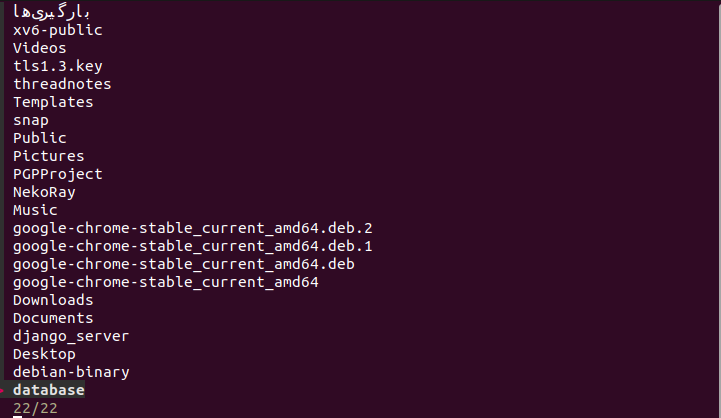
\includegraphics[width=0.8\textwidth, height=0.7\textheight]{assets/pictures/filtering_using_fzf.png}
                \caption{Interactive filtering of files and directories using \texttt{fzf}.}
            \end{figure}

            \textbf{Benefits of \texttt{ls | fzf} :}
            \begin{itemize}
                \item Simplifies navigation in large directories.
                \item Reduces time spent searching for files manually.
                \item Provides a responsive and interactive experience.
            \end{itemize}

            
            \subsubsection{Using \texttt{fzf} to Find Your Favorite PDF}

                You might have come across moments when you want to open up a certain PDF when studying for your final exams but finding the directory of that PDF is a very tiresome process. In this section, we will be using \texttt{fzf} to find our PDF in seconds! We will go step-by-step on how to find your file and use \texttt{fzf} to select it.
                
                \begin{enumerate}
                    \item First, we list the directory of all the files with the extension \texttt{.pdf}. The following command was used:
                    \begin{lstlisting}[language=bash]
                    fd -e pdf
                    \end{lstlisting}
                    \item Next, we used \texttt{fzf} to filter and select the desired PDF interactively. Here’s the command:
                    \begin{lstlisting}[language=bash]
                    fd -e pdf | fzf
                    \end{lstlisting}
                \end{enumerate}
                
                \textbf{Results :}
                
                \begin{figure}[H]
                    \centering
                    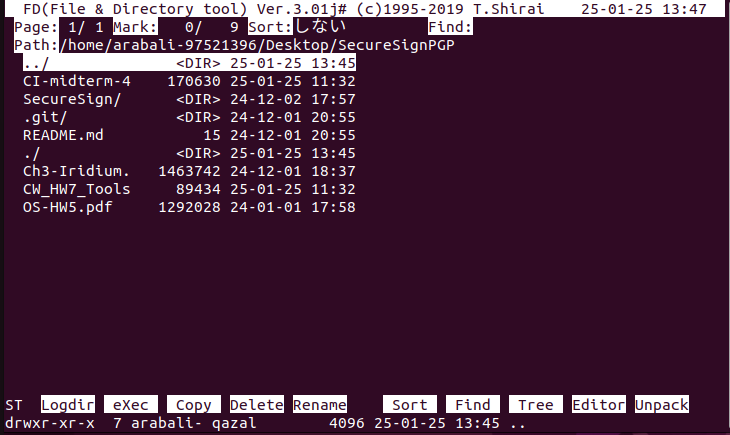
\includegraphics[width=\textwidth]{assets/pictures/find_desired_pdf.png}
                    \caption{Interactive filtering to find desired PDF \texttt{fzf}.}
                \end{figure}
                
            \subsubsection{Opening the File Using Zathura}
                
                Once we selected the desired PDF file, we used the minimalist program \texttt{Zathura} to open it. Here’s the command that accomplishes this:
                
                \begin{lstlisting}[language=bash]
                zathura $(fd -e pdf | fzf)
                \end{lstlisting}
                
                \textbf{Results :}
                
                \begin{figure}[H]
                    \centering
                    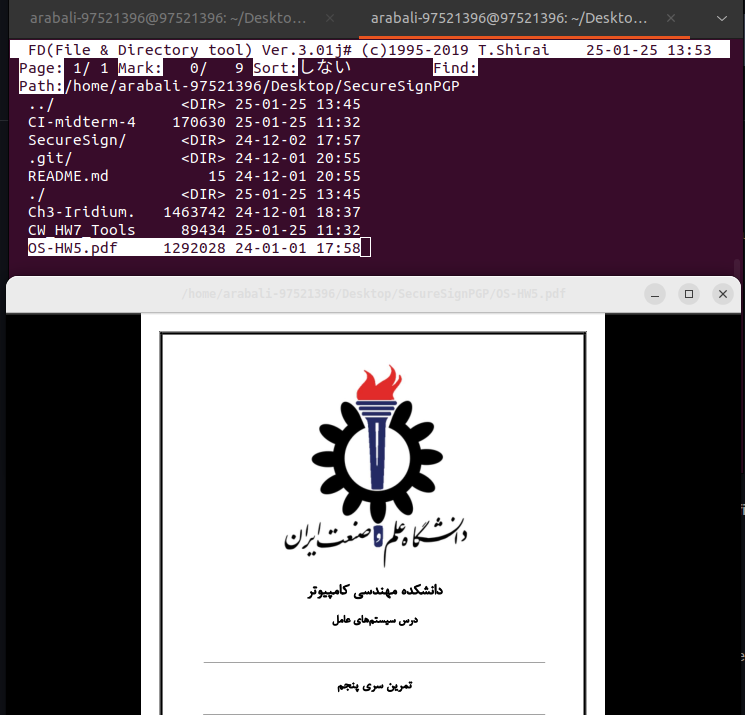
\includegraphics[width=\textwidth]{assets/pictures/find_and_open_desired_pdf.png}
                    \caption{Opening the selected PDF file using \texttt{Zathura}.}
                \end{figure}
            
                \vspace{1cm}

\section{Git and FOSS}
    \subsection{README.md}

        The \texttt{README.md} file for the repository serves as an introductory guide to the project. It provides an overview of the project’s purpose, key objectives, and usage instructions. The file includes details about repository structure, key features like automation workflows and exploration tasks, and a section encouraging contributions to the project.

        In this assignment, the \texttt{README.md} outlines :
        \begin{itemize}
            \item The integration of Git, GitHub, and LaTeX for effective workflow management.
            \item The repository structure, including the \texttt{CW\_Final\_Assignment.tex} file and supporting scripts.
            \item Key features explored, such as advanced Vim techniques, memory profiling using Valgrind, and CLI tools like \texttt{fzf}.
            \item A concise guide on how to clone and use the repository.
        \end{itemize}

        The \texttt{README.md} was created and committed to the repository following the guidelines provided in the assignment, ensuring clear communication of the repository’s purpose and contents.

        \vspace{1cm}

        \subsection{Issues}

            To fulfill the assignment's requirement, a sample issue was created in the GitHub repository, emphasizing the addition of contribution guidelines for better collaboration. This issue highlights the need for a \texttt{CONTRIBUTING.md} file to guide contributors on how they can participate in the project effectively.

            The following steps were performed :
            \begin{enumerate}
                \item Navigated to the \textbf{Issues} tab in the GitHub repository.
                \item Clicked on \textbf{New Issue} and provided a descriptive title and details for the issue.
                \item Submitted the issue, making it available for contributors to address.
            \end{enumerate}

            The created issue is displayed below :

            \begin{figure}[H]
                \centering
                
\includegraphics[width=0.8\textwidth]{assets/pictures/Requestـtoـaddـcontributionـguidelines.png}
                \caption{Created issue in the GitHub repository : Request to add contribution guidelines (Step 1).}
            \end{figure}

            \begin{figure}[H]
                \centering
                
\includegraphics[width=0.8\textwidth]{assets/pictures/Detailedـviewـofـtheـissue.png}
                \caption{Created issue in the GitHub repository : Detailed view of the issue (Step 2).}
            \end{figure}

            This demonstrates practical use of GitHub issues for project management and fostering collaboration in open-source projects.

        \subsection{FOSS Contribution}

            Free and Open Source Software (FOSS) projects play a critical role in the development of technology and knowledge sharing. I see myself contributing to FOSS projects in the future due to their impact on both personal and professional growth. 
            
            Here are some areas I am interested in contributing to :
            \begin{itemize}
                \item \textbf{Developer Tools:} Enhancing tools like text editors, compilers, or version control systems to improve the developer experience.
                \item \textbf{Machine Learning Libraries:} Contributing to popular libraries such as \texttt{TensorFlow} or \texttt{PyTorch} by implementing new features or optimizing existing ones.
                \item \textbf{Documentation:} Writing or improving documentation for FOSS projects to make them more accessible to beginners and advanced users alike.
                \item \textbf{Community Engagement:} Helping with issue tracking, bug fixes, and guiding new contributors to get started with FOSS projects.
            \end{itemize}
            
            The open-source community provides an excellent opportunity to learn, share knowledge, and collaborate with developers worldwide. Through these contributions, I aim to not only enhance my skills but also give back to the community that has provided numerous tools and resources that I use daily.
            
        \section*{Submission Guidelines}

            The final submission for the assignment includes the following :
            
            \begin{itemize}
                \item \textbf{Link to the GitHub repository:} \href{https://github.com/qazalarabali/CW_Final_Assignment}{CW\_Final\_Assignment on GitHub}.
                \item \textbf{Compiled PDF of the LaTeX document:} 
                    \begin{itemize}
                        \item The PDF is available as an \textbf{Artifact} generated automatically by GitHub Actions for intermediate updates.
                        \item The PDF is also available as part of a \textbf{Release} for finalized versions of the document.
                    \end{itemize}
                \item \textbf{All source files:} All scripts, workflows, and additional files used during the creation of the document and project are included in the repository.
            \end{itemize}
            
\end{document}
